\documentclass[14pt, a4paper]{article}

\usepackage[utf8]{inputenc}
\usepackage[T2A]{fontenc}

\usepackage{graphicx}
\graphicspath{ {image/} }

\usepackage{amsmath}

\tolerance 1414
\hbadness 1414
\emergencystretch 1.5em
\hfuzz 0.3pt        % размер максимального переполнения без warning'a
\widowpenalty=10000 % запрещает одиночную строку абзаца в начале страницы 
\vfuzz \hfuzz
\raggedbottom       % если на странице мало содержимого, добавить пустое место в конце, а не в середине страницы



\title{Курсовая работа по электротехнике. Часть 1}
\author{Новоженов П.А. ЭН-26}
\date{}

\begin{document}

\maketitle

\newpage

\section*{Схема в мультисиме}

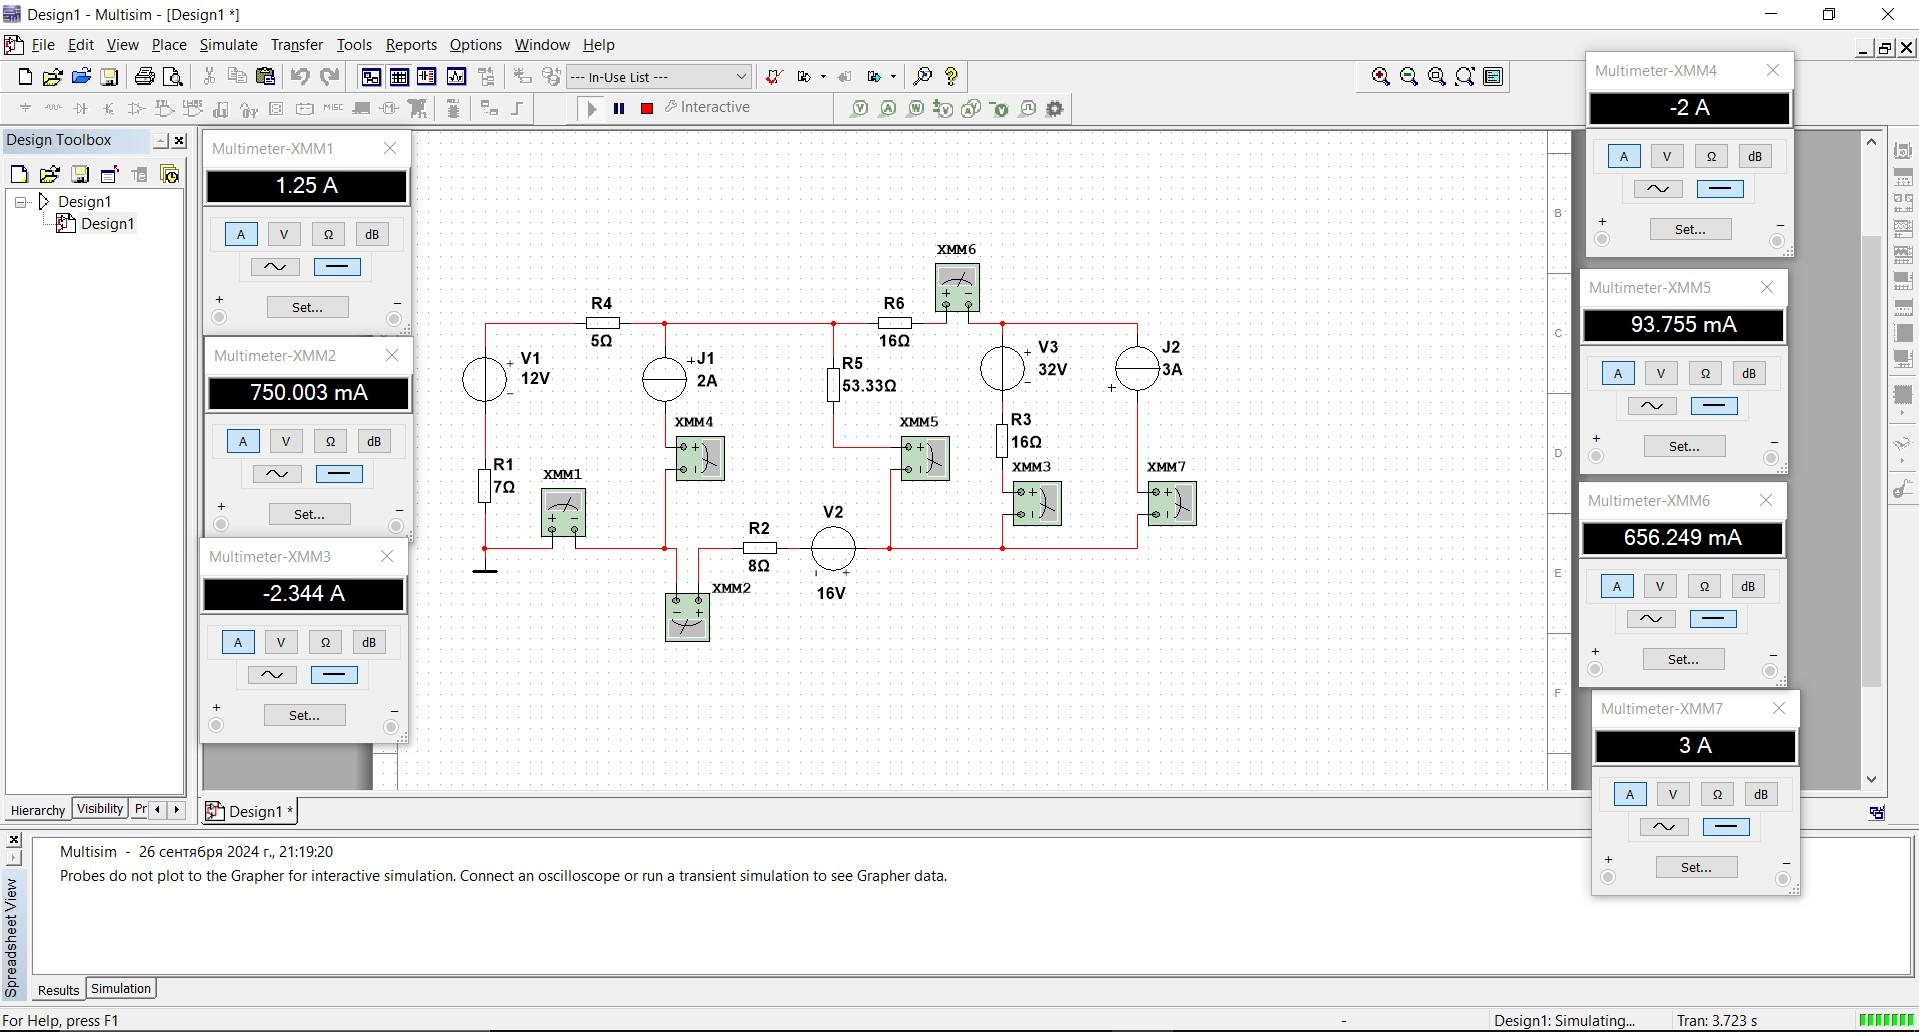
\includegraphics[width=1\textwidth]{Full_design.jpg}


\section*{Метод эквивалентных преобразований}

    \subsection*{Шаг 1}

    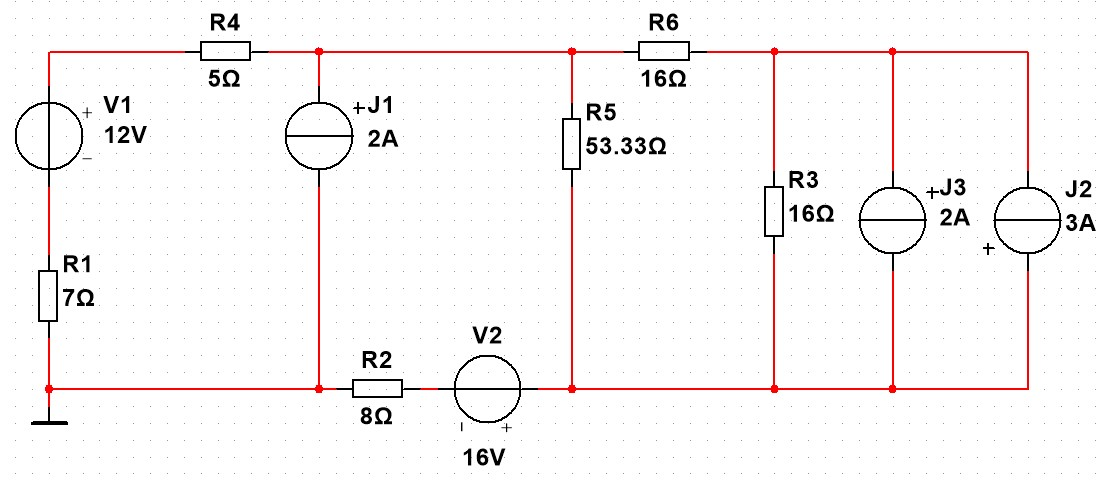
\includegraphics[width=1\textwidth]{Stage1.jpg}
    $$J_3 = \frac{E_3}{R_3} = \frac{32}{16} = 2 \ A$$

    \subsection*{Шаг 2}
    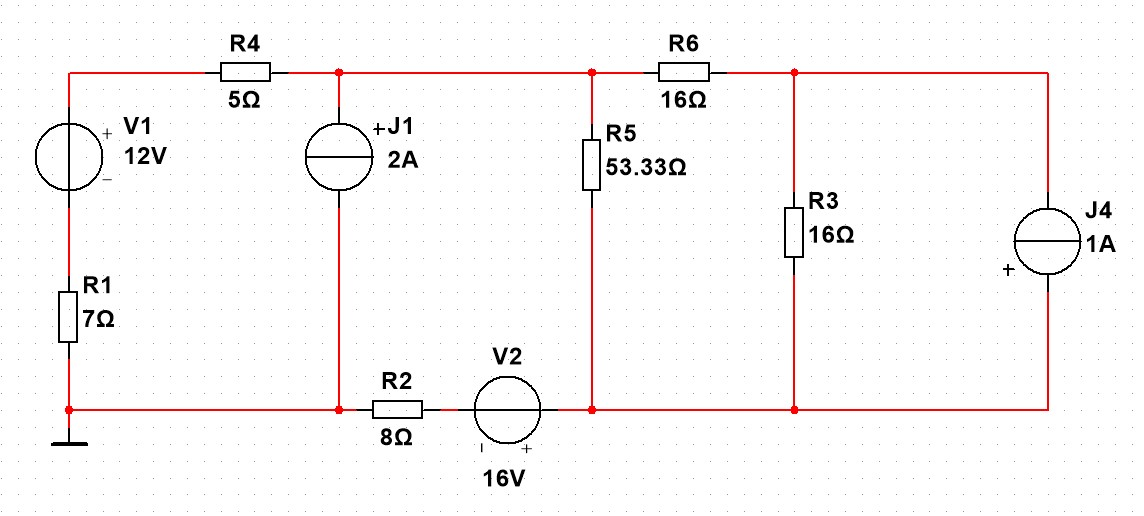
\includegraphics[width=1\textwidth]{Stage2.jpg}
    $$J_4 = J_2 - J_3 = 3 - 2 = 1 \ A$$

    \subsection*{Шаг 3}
    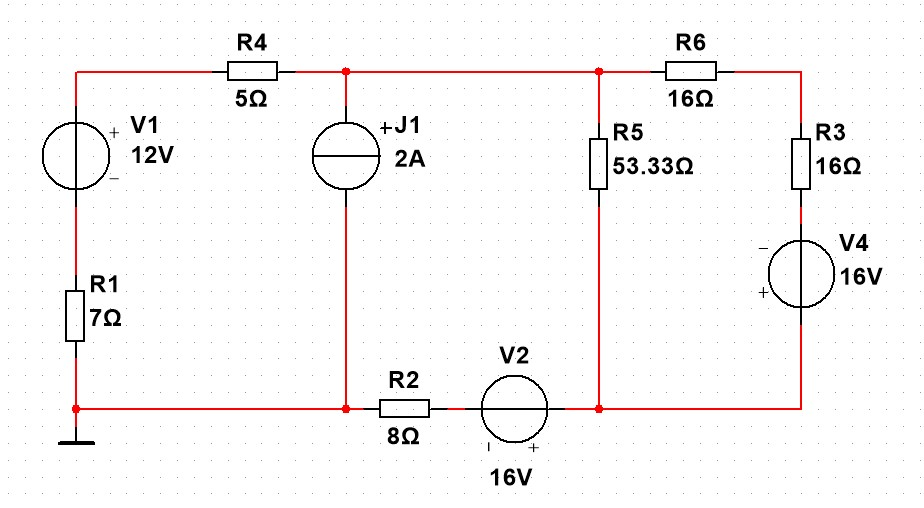
\includegraphics[width=1\textwidth]{Stage3.jpg}
    $$E_4 = J_4 R_3 = 1 \cdot 16 = 16 \ V$$

    \subsection*{Шаг 4}
    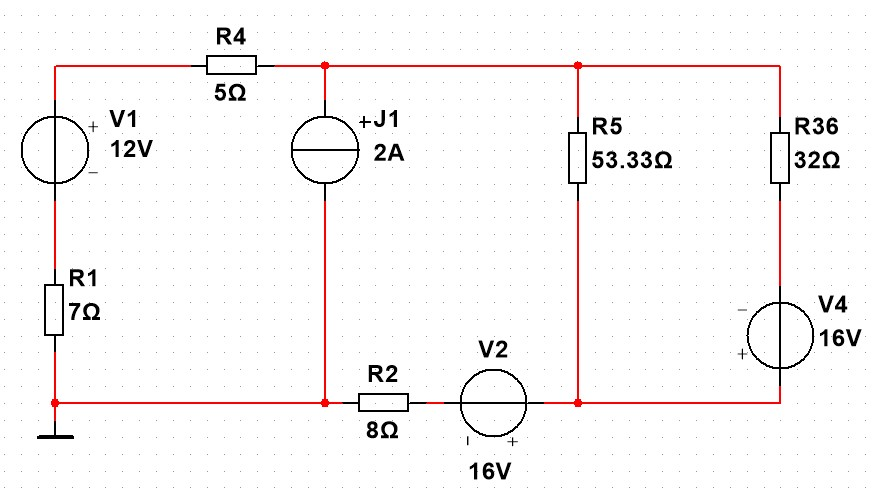
\includegraphics[width=1\textwidth]{Stage4.jpg}
    $$R_{36} = 32 \ \Omega$$


    \subsection*{Шаг 5}
    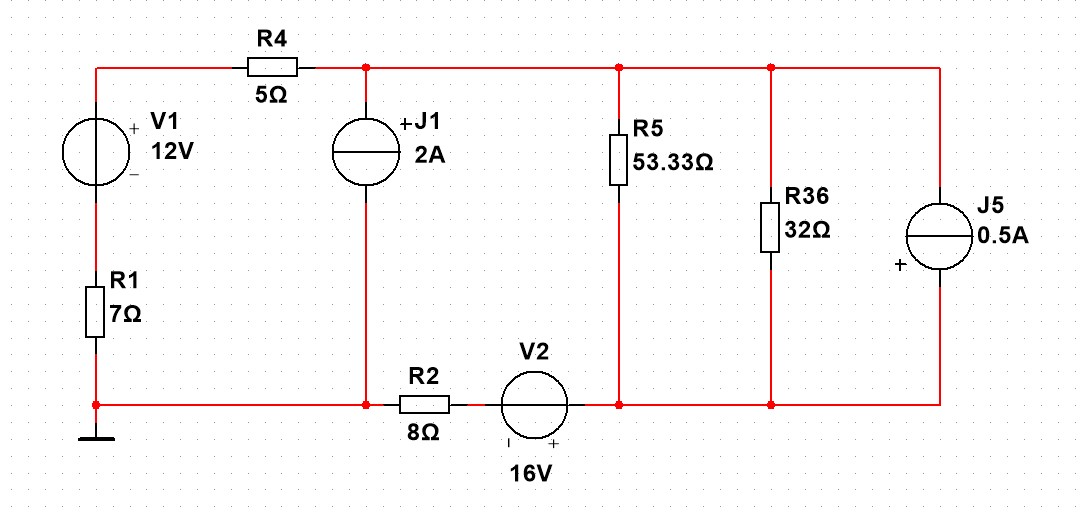
\includegraphics[width=1\textwidth]{Stage5.jpg}
    $$J_5 = \frac{E_4}{R_{36}} = \frac{16}{32} = 0.5 \ A$$

    \subsection*{Шаг 6}
    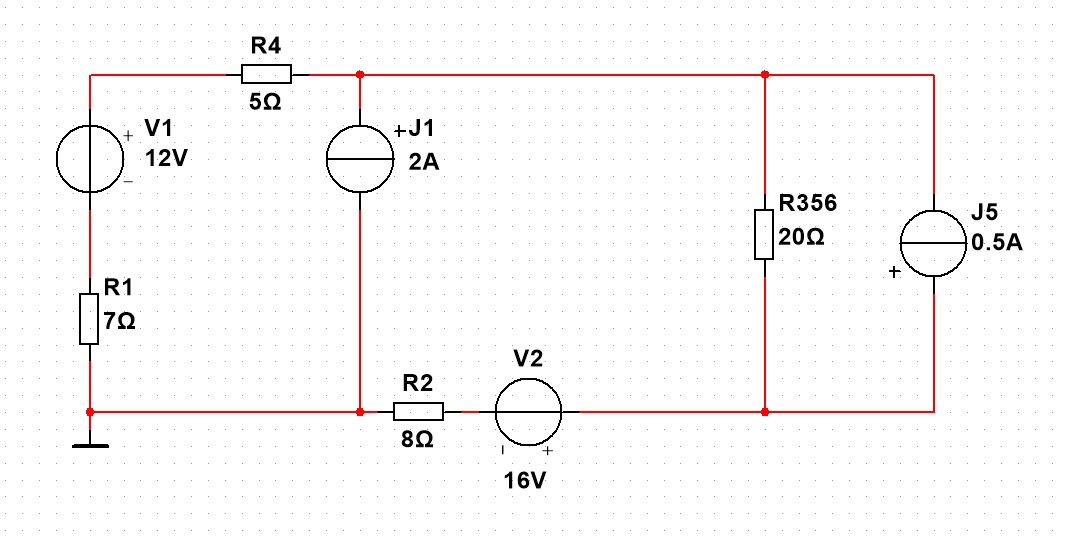
\includegraphics[width=1\textwidth]{Stage6.jpg}
    $$R_{356} = \frac{R_{36} \cdot R_5}{R_{36} + R_5} = \frac{32 \cdot 53.33}{32 + 53.33} = 20 \ \Omega$$

    \subsection*{Шаг 7}
    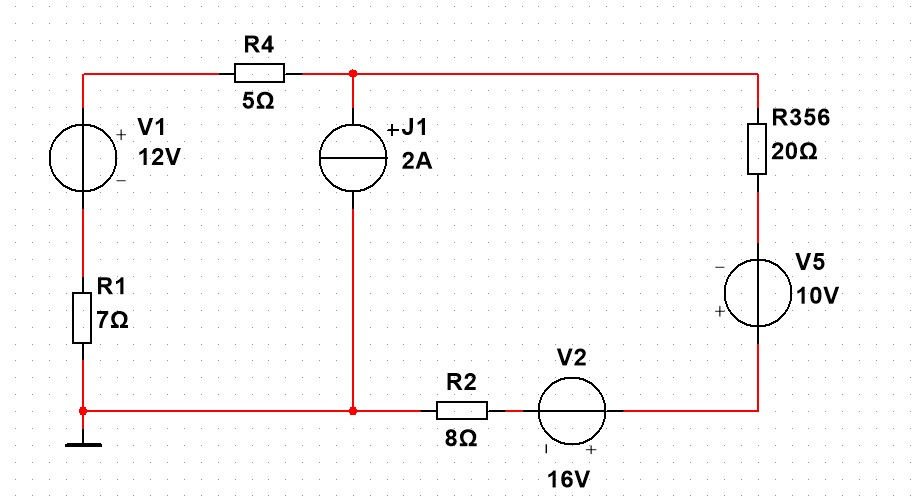
\includegraphics[width=1\textwidth]{Stage7.jpg}
    $$E_5 = J_5 R_{356} = 0.5 \cdot 20 = 10 \ V$$

    \subsection*{Шаг 8}
    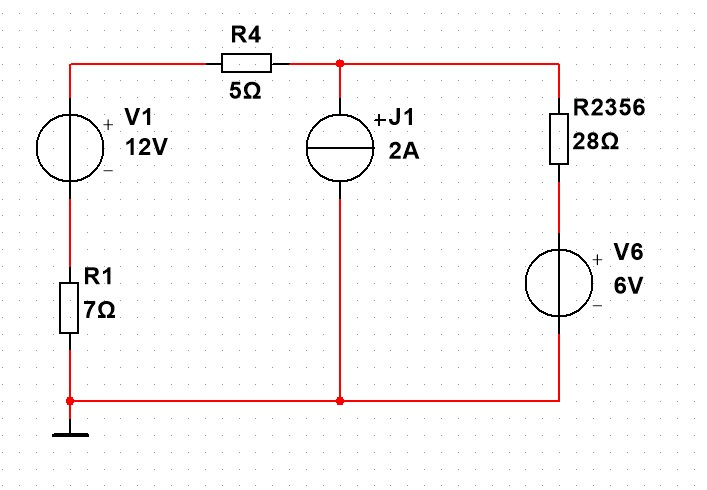
\includegraphics[width=1\textwidth]{Stage8.jpg}
    $$E_6 = E_2 - E_5 = 6 \ V$$
    $$R_2356 = R_2 + R_{356} = 8 + 20 = 28$$

    \subsection*{Шаг 9}
    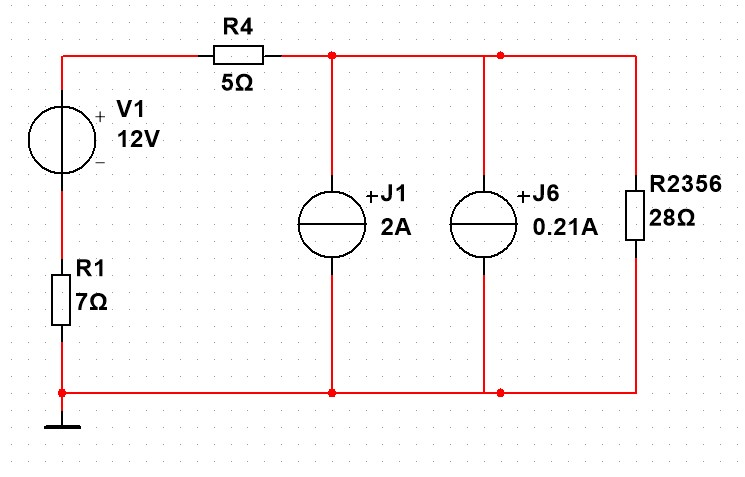
\includegraphics[width=1\textwidth]{Stage9.jpg}
    $$J_6 = \frac{E_6}{R_{2356}} = \frac{6}{28} = 0.21 \ A$$

    \subsection*{Шаг 10}
    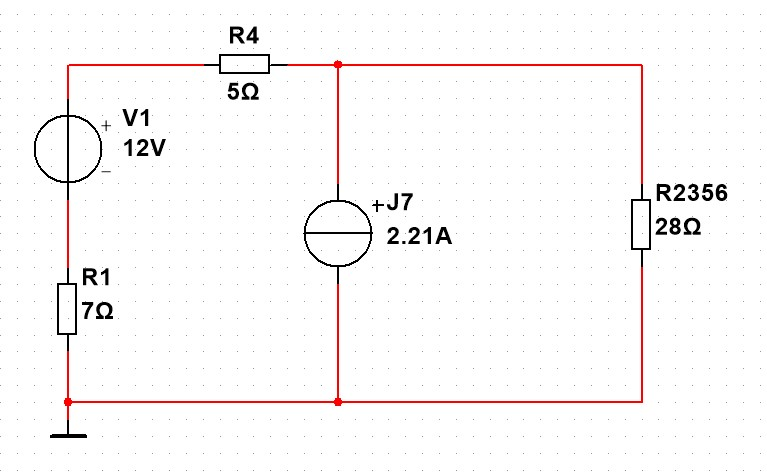
\includegraphics[width=1\textwidth]{Stage10.jpg}
    $$J_7 = J_1 + J_6 = 2.21 \ A$$

    \subsection*{Шаг 11}
    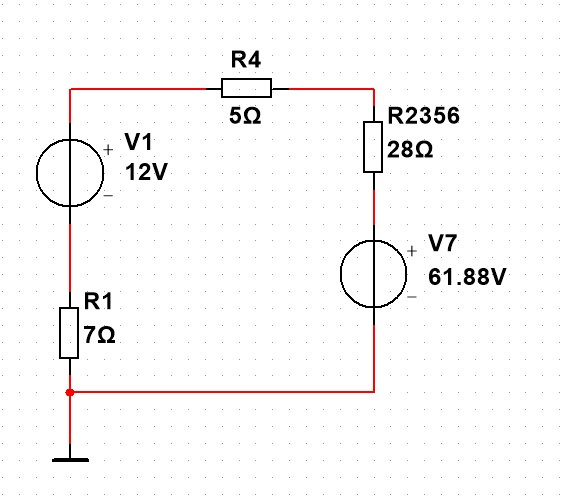
\includegraphics[width=1\textwidth]{Stage11.jpg}
    $$E_7 = J_1 R_{2356} = 2.21 \cdot 28 = 61.88 \ V$$

    \subsection*{Шаг 12}
    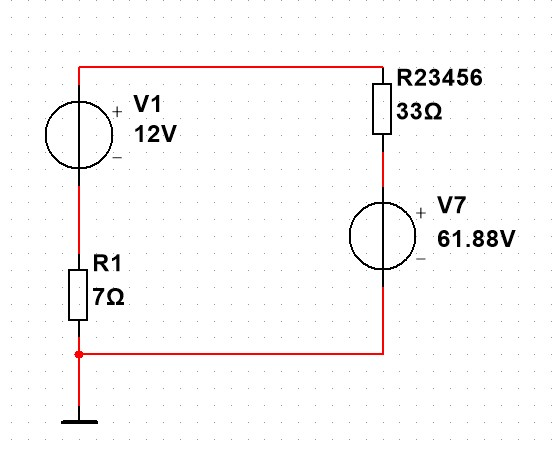
\includegraphics[width=1\textwidth]{Stage12.jpg}
    $$R_{23456} = R_4 + R_{2356} = 5 + 28 = 33 \ \Omega$$

    \subsection*{Шаг 13}
    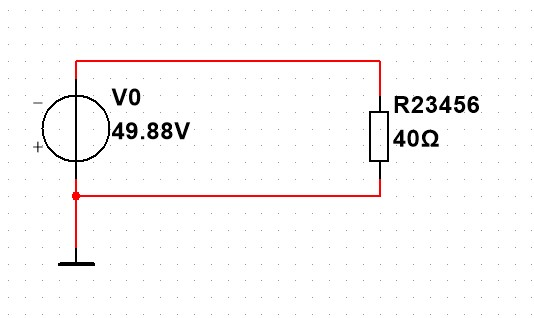
\includegraphics[width=1\textwidth]{Stage13.jpg}
    $$E_0 = E_7 - E_1 = 61.88 - 12 = 49.88 \ V$$
    $$R_0 = R_{23456} + R_1 = 33 + 7 = 40 \ \Omega$$

    \subsection*{Шаг 14}
    $$I_{R_1} = \frac{E_0}{R_0} = \frac{49.88}{40} = 1.25 \ A$$

\section*{Метод непосредственного применения законов Кирхгофа}

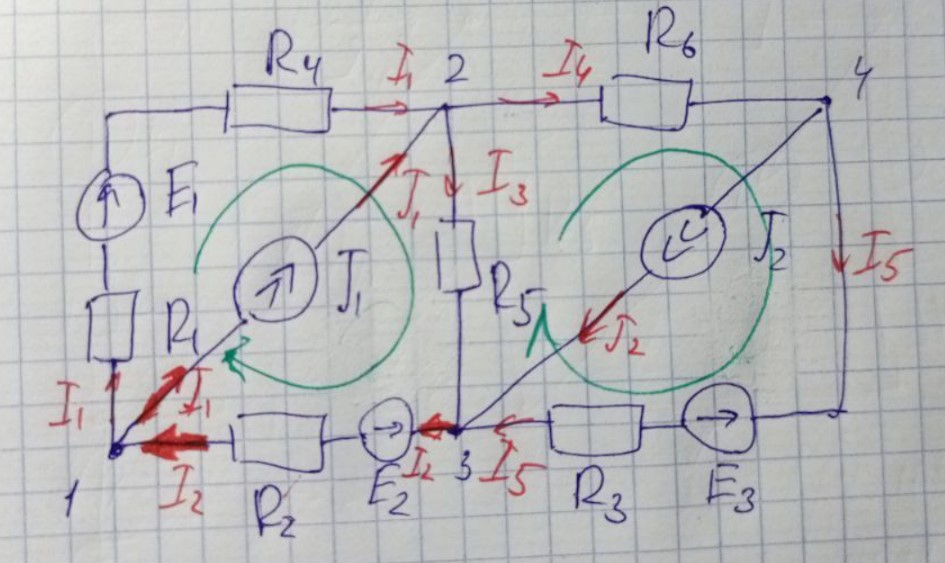
\includegraphics[width=1\textwidth]{kirh.jpg}

    Запишем уравнения по I закону Кирхгофа.
    $$1: \ I_2 = I_1 + J_1$$
    $$2: \ I_1 + J_1 = I_3 + I_4$$
    $$3: \ I_3 + I_5 + J_2 = I_2$$

    Запишем систему уравнений из этих трех уравнений и II законов Кирхгофа подставив значения $J_1$ и $J_2$.
    $$\begin{aligned}
    I_1 - I_2 = -2 \\
    I_1 - I_3 - I_4 = -2 \\
    -I_2 + I_3 + I_5 = -3 \\
    R_6I_4 + I_5R_3 - I_3R_5 = -32 \\
    (R_1+R_4)I_1 + R_2I_2 + R_5I_3 = -4
    \end{aligned}.$$

    Представим систему в матричном виде:
    $$\begin{pmatrix} 
    1 & -1 & 0 & 0 & 0 & | -2  \\ 
    1 & 0 & -1 & -1 & 0 & | -2 \\ 
    0 & -1 & 2 & 0 & 1 & | -3 \\ 
    0 & 0 & -53.33 & 16 & 16 & | -32 \\ 
    12 & 8 & 53.33 & 0 & 0 & | -4
    \end{pmatrix}$$

    Решение СЛАУ выглядит так:
    $$\begin{pmatrix}  
    I_1  \\ 
    I_2 \\ 
    I_3 \\ 
    I_4 \\ 
    I_5
    \end{pmatrix} = 
    \begin{pmatrix}
    -1.250 \\ 
    0.750 \\ 
    0.094 \\ 
    0.656 \\ 
    -2.344
    \end{pmatrix}
    $$

\section*{Метод контурных токов}

    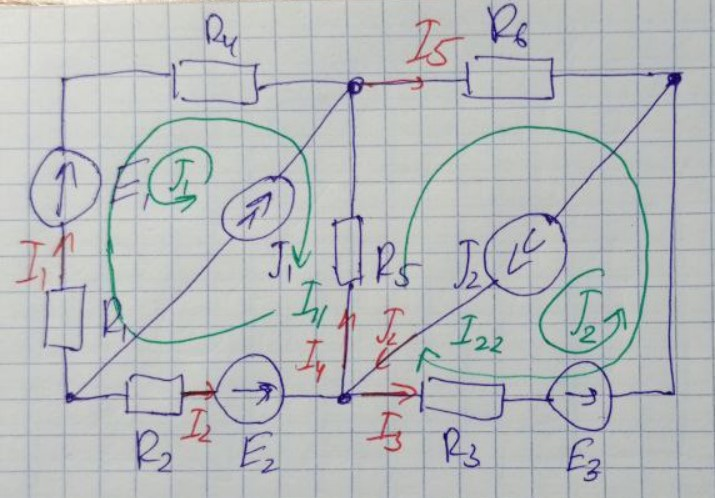
\includegraphics[width=1\textwidth]{MKT.jpg}

    Выразим каждый ток ветви через контурные токи:
    $$I_1 = I_{11}-J_1$$
    $$I_2 = - I_22$$
    $$I_3 = J_2 - I_22$$
    $$I_4 = I_{22} - I_{11}$$
    $$I_5 = I_{11}$$

    Напишем II закон Кирхгофа для двух контуров, с учетом выведенных на лекции правил:
    $$-(R_1+R_4)J_1 + (R_1 + R_2 + R_4)I_{11} - R_5I_{22} = E_1 - E_2$$
    $$-(R_5)I_{11} + (R_3 + R_5 + R_6)I_{22} - R_3J_2 = -E_3$$

    Составим из этих уравенений СЛАУ в матричном виде:
    $$
    \begin{pmatrix}
        73.33 & -53.33 & | 20 \\
        -53.33 & 85.33 & | 16
    \end{pmatrix}
    $$

    Решением этой слау будет:
    $$
    \begin{pmatrix}
        I_{11} \\ I_22
    \end{pmatrix} = 
    \begin{pmatrix}
       0.75  \\ 0.656
    \end{pmatrix}
    $$

    Теперь найдем все токи:
        $$I_1 = -1.25 \ A$$
        $$I_2 = -0.75 \ A$$
        $$I_3 = 2.344 \ A$$
        $$I_4 = -0.094 \ A$$
        $$I_5 = 0.656$$

\section*{Баланс мощностей}
    Сумма мощностей источников напряжения:
    $$\sum E_k I_k = -E_1I_1 + -E_2I_2 + E_3I_5 = -15  - 12 + 75 = 48$$
    Сумма мощностей источников тока:
    $$\sum U_k J_k = ([R_1 + R_4]I_1 + E_1)J_1 + (I_5R_3 - E_3)J_2 = 54 + 16.5 = 70.5$$
    Сумма мощностей выделяющихся на сопростивлениях:
    $$\sum I_k^2 R_k = I_1^2(R_1 + R_4) + I_2^2R_2 + I_3^2R_5 + I_4^2 R_6 + I_5^2 R_3 =\dots $$
    $$ \dots= 18.75 + 4.5 + 0.47 + 6.8 + 87.9 = 118.42$$

    Получается:
    $$\sum E_k I_k + \sum U_k J_k = \sum I_k^2 R_k$$
    $$48 + 70.5 = 118.5 = 118.42$$
    
    Не совпадение в $0.08$ можно считать незначительным. Появилось оно, скорее всего, из-за дробного значения $R_5$ и
    округления промежуточных значений.
    
\section*{Метод узловых потенциалов}
    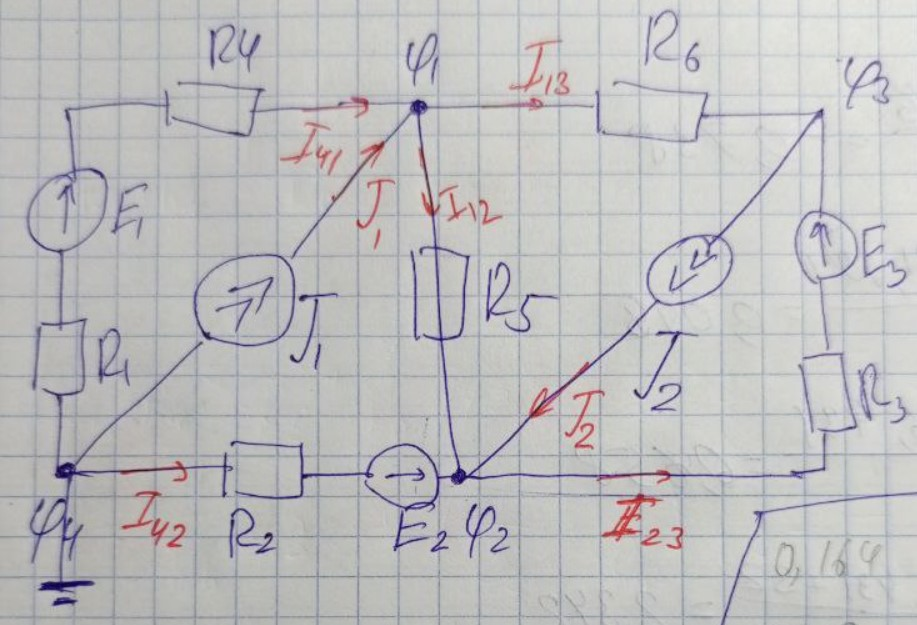
\includegraphics[width=1\textwidth]{myp.jpg}

    Распишем I закон Кирхгофа для первых трех потенциалов:
    $$I_{41} + J_1 = I_{12} + I_{13}$$
    $$I_{42} + I_{12} + J_2 = I_23$$
    $$I_{13} + I_{23} = J_2$$

    Выразим каждый ток через расширенный закон Ома:
    $$I_{41} = \frac{\varphi_4 - \varphi_1 + E_1}{R_1 + R_4}$$
    $$I_{42} = \frac{\varphi_4 - \varphi_2 + E_2}{R_2}$$
    $$I_{12} = \frac{\varphi_1 - \varphi_2}{R_5}$$
    $$I_{13} = \frac{\varphi_1 - \varphi_3}{R_6}$$
    $$I_{23} = \frac{\varphi_2 - \varphi_3 + E_3}{R_3}$$


    Подставим выраженные токи в первые три уравнения:
    $$\frac{\varphi_4 - \varphi_1 + E_1}{R_1 + R_4} + J_1 = \frac{\varphi_1 - \varphi_2}{R_5} + \frac{\varphi_1 - \varphi_3}{R_6}$$
    $$\frac{\varphi_4 - \varphi_2 + E_2}{R_2} + \frac{\varphi_1 - \varphi_2}{R_5} + J_2 = I_{23} = \frac{\varphi_2 - \varphi_3 + E_3}{R_3}$$
    $$\frac{\varphi_1 - \varphi_3}{R_6} + \frac{\varphi_2 - \varphi_3 + E_3}{R_3} = J_2$$

    Представим эти уравнения в форме:
    $$(\frac{1}{R_1 +R_4} + \frac1{R_5} + \frac1{R_6}) \varphi_1 - \frac{1}{R_5}\varphi_2 - \frac1{R_6}\varphi_3 = \frac{E_1}{R_1 + R_4} + J_1$$
    $$-\frac1{R_5}\varphi_1 + (\frac1{R_2} + \frac1{R_3} + \frac1{R_5})\varphi_2 - \frac1{R_3}\varphi_3 = \frac{E_2}{R_2} - \frac{E_3}{R_3} + J_2$$
    $$-\frac1{R_6}\varphi_1 - \frac1{R_3}\varphi_2 + (\frac1{R_6} + \frac1{R_3})\varphi_3 = \frac{E_3}{R_3} - J_2$$

    Получим систему уравнений:
    $$
    \begin{pmatrix}
        0.164 & -0.018 & -0.0625 & | + 3 \\
        -0.018 & 0.206 & -0.0625 & | + 3 \\
        -0.0625 & -0.0625 & 0.125 & | -1
    \end{pmatrix}
    $$

    Решение этой системы:
    $$
    \begin{pmatrix}
        \varphi_1 \\ \varphi_2 \\ \varphi_3
    \end{pmatrix} = 
    \begin{pmatrix}
        26.959 \\ 21.904 \\ 16.431
    \end{pmatrix}
    $$

    Найдем все токи, по формулам выше:

    $$I_{41} = -1.25 \ A$$
    $$I_{42} = -0.738 \ A$$
    $$I_{12} = 0.095 \ A$$
    $$I_{13} = 0.658 \ A$$
    $$I_{23} = 2.342 \ A$$

\section*{Потенциальная диаграмма}

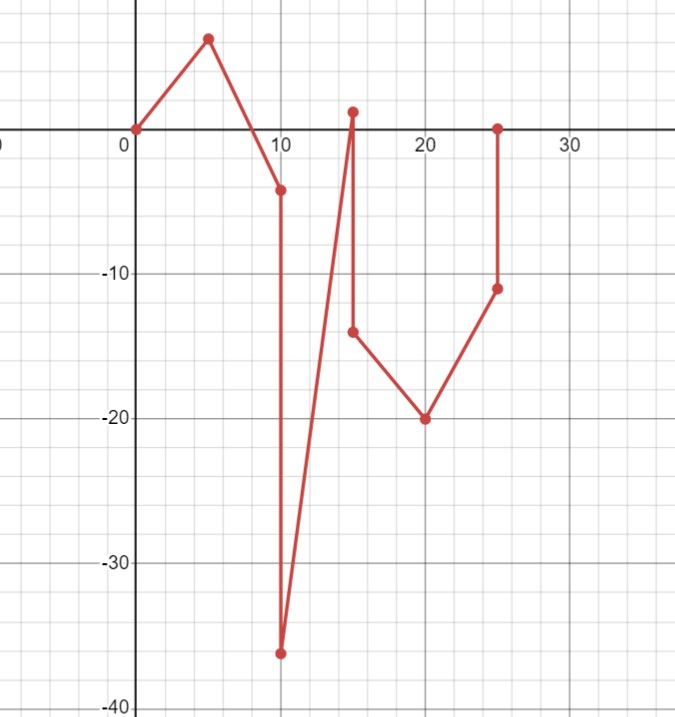
\includegraphics[width=1\textwidth]{diagram.jpg}

Потенциальная диаграмма не сходится на 0.04 вольта. Эта разница возникает 
из-за дробного значения $R_5$ и округления промежуточных величин.

\section*{Таблица с итогами}

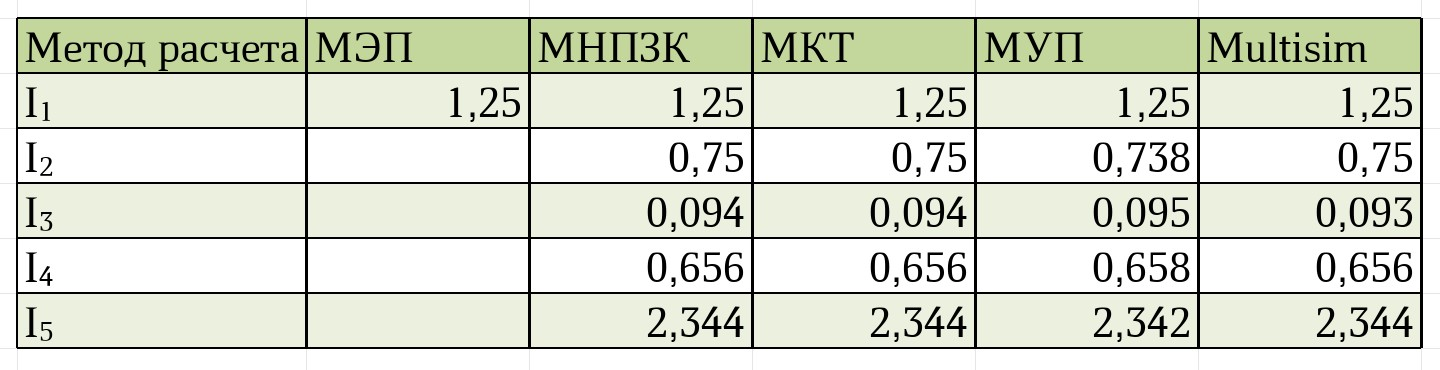
\includegraphics[width=1\textwidth]{result.jpg}


\end{document}
